\documentclass[10pt]{article}
\usepackage[utf8]{inputenc}
\usepackage[T1]{fontenc}
\usepackage{graphicx}
\usepackage[export]{adjustbox}
\graphicspath{ {./images/} }
\usepackage{amsmath}
\usepackage{amsfonts}
\usepackage{amssymb}
\usepackage[version=4]{mhchem}
\usepackage{stmaryrd}
\usepackage{bbold}

\begin{document}
\begin{center}
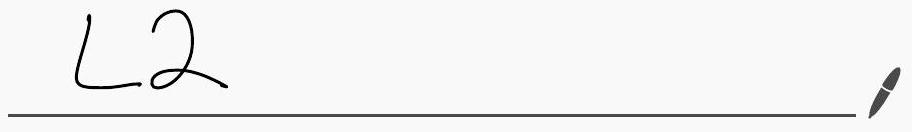
\includegraphics[max width=\textwidth]{2025_09_02_1faef23cd03b7ec5e264g-01}
\end{center}

\section*{L2: Prime Numbers}
Definition: Let $p \in \mathbb{Z}$ with $p>1$. Then $p$ is said to be a prime if the only positive divisors of $p$ are 1 and $p$. If $n \in \mathbb{Z}, n>1$, and $n$ is not prime, then $n$ is said to be composite.

\begin{itemize}
  \item The positive integer 1 is neither prime non composite. We will give a compelling reason for this later in the course.\\
Example: The prime numbers between 2 and 50 are $2,3,5,7,11,13,17,19,23,29,31,37,41,43$, and 47. All primes except 2 are odd.\\
Lemma 1.5: Every integer greater than 1 has a prime divisor.\\
Proof: Assume there exists an integer $n>1$ that has no prime divisor. By the well ordering principle we may assume that $n$ is the least such integer. Clearly $n \mid n$, so $n$ is not prime. Thus $n$ is Composite and Consequently there\\
exist $a, b \in \mathbb{Z}$ such that $n=a b$, where $1<a<n$ and $1<b<n$. Since $1<a<n$, we have that $a$ has a prime divisor, say $p$, so that $p l a$. But $a l n$, so we have that pln by Proposition 1.1 (transitivity of divisibility). Contradiction! Thus every integer greater than I has a prime divisor.\\
Theorem 1.6 (Enclid) There are infinitely many prime numbers.\\
Proof: Assume that there are only finitely many prime numbers, say $P_{1}, P_{2}, \ldots, P_{n}$. Consider the integer $N:=P_{1} P_{2} \ldots P_{n}+I$. By Lemma 1.5 we know that $N$ has a prime divisor, say $\rho$. Thus $p=p_{i}$ for some $i$, $i=1, \cdots, n$. Then $p \mid\left(N-p_{1} p_{2} \cdots p_{n}\right)$ by Proposition 1.2, so P|1, a contradiction. Thus there are infinitely many prime numbers.
\end{itemize}

Proposition 1.7: Let $n$ be a composite number. Then $n$ has a prime dividor $p$ with $p \leq \sqrt{n}$. Proof: Since $n$ is composite, there exist $a, b \in \mathbb{Z}$ such that $n=a b, 1<a<n, 1<b<n$, and without loss of generality, $a \leq b$. We must have $a \leqslant \sqrt{n}$, otherwise if $a>\sqrt{n}$ we have $n=a b>\sqrt{n} \sqrt{n}=n$, which is not possible.\\
By Lemma 1.5 we know that a must have a prime divisor, say $p$. Since $p l a$ and $a l n$ we have pln by Proposition 1.1 (transitivity of divisibility). Furthermone, $p \leq a \leq \sqrt{n}$, so $p$ is the desired prime factor of $n$.

\begin{itemize}
  \item Proposition 1.7 gives a method for finding all the prime numbers less than or equal to a specified integer $n>1$ This is called the sieve of Eratosthenes.\\
Example: Suppose one wants to find all the primes less than 50. By Proposition 1.7\\
any composite number less than 50 must have a prime dividor less than or equal to $\sqrt{50} \approx 7.07$ i.e. $2,3,5,7$. Deleting all multiples of these primes (except for themselves) gives:\\
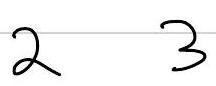
\includegraphics[max width=\textwidth, center]{2025_09_02_1faef23cd03b7ec5e264g-05}\\
$\begin{array}{llllllllll}11 & 12 & 13 & 14 & 18 & 16 & 17 & 18 & 19 & 26\end{array}$\\
21 22 23 24 25 26 27 28 29 30\\
$31 \quad 32 \quad 35 \quad 34 \quad 35 \quad 36 \quad 37 \quad 38 \quad 39 \quad 46$\\
$41 \quad 42 \quad 43 \quad 44 \quad 45 \quad 46 \quad 47 \quad 48 \quad 49 \quad 50$\\
Remaining numbers are prime:\\
$2,3,5,7,11,13,17,19,23,29,31,37,41$,\\
$43,47$.
  \item Proposition 1.7 gives a very crude primality test i.e. an algorithm to test whether a given $n>1$ is prime or composite\\
i.e. Check whether $n$ is divisible by any prime number $p \leq \sqrt{n}$. If $n$ is divisible by such a prime, then $n$ is composite. Otherwise, $n$ is
\end{itemize}

\section*{prime.}
\begin{itemize}
  \item We will discuss more efficient primality tests later in the course.
  \item If one does larger experiments with the sieve of Eratos thenes one might guess that the primes are more sparsely distributed as you progress through larger and larger integers. The next Proposition shows that there exist arbitrarily long sequences of Consecutive positive integers that don't Contain Prime numbers\\
Proposition 1.8: For any positive integer $n$, there are at least $n$ consecutive composite positive integers.\\
Proof: Given $n \geqslant 1$, consider the sequence
\end{itemize}

$$
(n+1)!+2,(n+1)!+3, \cdots,(n+1)!+n+1 .
$$

Let $i$ be an integer such that $2 \leq i \leq n+1$. Since $i|(n+1)|$ and $i \mid i$, we have $i|(n+1)|+i$ for $2 \leq i \leq n+1$, by Proposition 1.2. Thus each integer in the sequence is composite.

\begin{itemize}
  \item It also seems that one can find primes (6) very close to one another\\
i.e. $(3,5),(5,7),(11,13), \ldots$\\
A pair ( $P, P+2$ ) with both entries prime are called twin primes.\\
Conjecture: There are infinitely many prime numbers $P$ for which $P+2$ is also Prime.
  \item There has been very recent breakthroughs on this problem. Let $p_{1}, p_{2}, \ldots$ denote the sequence of primes. Zhang (2013) proved that there are infinitely many primes $p_{n}$ such that $P_{n+1}-P_{n} \leqslant 70000000$. This has been improved by others, Maynard, Tao, $\cdots$, but not all the way to 2 .\\
One of the most famous (and classical) results about the Primes is the Prime Number Theorem (PNT). This was conjectured by Gauss in 1793 and was proved independently\\
in 1896 by C.J. de la Vallée Poussin 7 and J. Hadamard. The PNT gives an estimate for the number of primes up to a real positive number $x$.\\
Definition: Let $x \in \mathbb{R}$ with $x>0$. Then
\end{itemize}

$$
\pi(x):=\mid\{p: p \text { prime; } \mid<p \leqslant x\} \mid \text {. }
$$

Theorem 1.9 (PNT): $\lim _{x \rightarrow \infty} \frac{\pi(x)}{x / \log x}=I$.

\begin{itemize}
  \item Theorem 1.9 is equivalent to saying that $\pi(x)$ may be approximated by $\frac{x}{\log x}$ as $x \rightarrow \infty$.
  \item The proof of PNT is beyond the scope of this class (requires Complex analysis and more advanced number theory).\\
Many unsolved problems in number theory deal with integers that are expressible in certain forms.
\end{itemize}

\section*{Conjecture (Goldbach, 1742):}
Every even integer greater than 2 can be expressed as the sum of two (not necessarily distunct) prime numbers.\\
i.e. $4=2+2,6=3+3,8=3+5$, and so on

\begin{itemize}
  \item Goldbach's conjecture has been Verified experimentally up to some large finite point, but a proof still eludes the research community. In fuct, Hardy and Littlewood predicted a frmula for the number of representations an even integer has in terms of a sum of two primes. Still an open problem!
  \item We now consider other families of Primes and close with some more open conjectures.\\
Definition: Any prime number expressible in the form $2^{p}-1$ with $p$ prime is said to be a Mersenne prime.
\end{itemize}

Example: The first five Mersenne primes\\
are $3=2^{2}-1,7=2^{3}-1,31=2^{5}-1$,\\
$127=2^{7}-1$ and $8191=2^{13}-1$.\\
Note that $2^{\prime \prime}-1=2047=(23)(89)$ is not a Mersenne prime.\\
Conjecture: There are infinitely many Mersenne primes.

Another interesting family of prime numbers are due to Fermat.\\
Definition: Any prime number expressible in the form $2^{2^{n}}+1$ with $n \in \mathbb{Z}$ and $n \geqslant 0$ is said to be a Fermat Prime.\\
Example: The first five Fermat primes are $3=2^{2^{0}}+1,5=2^{2^{1}}+1,17=2^{2^{2}}+1$,\\
$257=2^{2^{3}}+1$, and $65537=2^{2^{4}}+1$.

\begin{itemize}
  \item Fermat in 1640 conjectured that any.\\
number expressible in the form $2^{2^{n}}+1$\\
with $n \in \mathbb{Z}$ and $n \geqslant 0$ is prime.
  \item Fermat's conjecture was disproved in 1732 by Enler who proved that $641 / 2^{2^{5}}+1$ i.e. $2^{2^{5}}+1$ is not a Fermat prime.
\end{itemize}

Conjecture: There are exactly five Fermat primes.

\begin{itemize}
  \item The last family we consider is due to Hardy and Littlewood 1922 :\\
Conjecture: There are infinitely many primes expressible in the form $n^{2}+1$ where $n$ is a positive integer.\\
Remark: In view of the above conjecture it may be tempting to conjecture there are infinitely many primes of the form $n^{2}-1$ for $n$ a positive integer. However,
\end{itemize}

$$
n^{2}-1=(n+1)(n-1),
$$

which rules out the primality of $n^{2}-1$ for\\
$n>2$. Factorisations can be a powerful (II) tool.


\end{document}